\documentclass[12pt,aspectratio=169]{beamer}

\usetheme[
    sectionpage=progressbar,
    subsectionpage=progressbar,
    progressbar=frametitle
]{metropolis}

\usepackage[utf8]{inputenc}
\usepackage[spanish]{babel}
\usepackage{amsmath}
\usepackage{graphicx}

\title{Introducción a la Optimización para Invertir en la Bolsa}
\author{Luis Biedma - lbiedma17@gmail.com}
\date{29/09/2018}

\begin{document}

\maketitle

\begin{frame}{Contenido}
	\tableofcontents
\end{frame}


\section{Optimización}
\begin{frame}{Introducción}
Imaginemos que tenemos que armar un desayuno nutritivo con los siguientes elementos:

\begin{center}
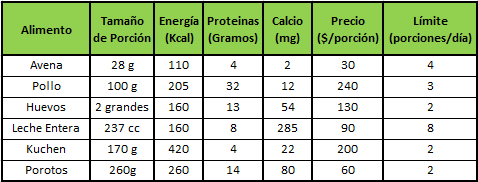
\includegraphics[width=.8\paperwidth]{desayuno.png}
\end{center}
\end{frame}

\begin{frame}{Introducción}
Un problema similar a éste tenía Leonid Kantorovich en los '40, en una escala un poquito más grande...

\begin{center}
\uncover<2>{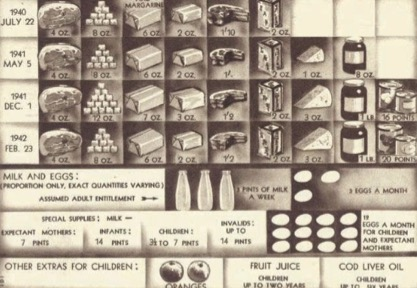
\includegraphics[width=.5\paperwidth]{rations.jpg}}
\end{center}
\end{frame}

\begin{frame}{Qué es la optimización?}

En criollo:
\begin{itemize}
\item Encontrar el \textbf{mejor valor} para una función (objetivo, costo, pérdida)...
\item ... relativo a algún conjunto (restricciones).

\end{itemize}

\uncover<2>{
Un poquito más formal:

$$
\min_x f(x)
$$
$$
sa \hspace{5pt} x \in S
$$
}
\end{frame}

\subsection{Aplicaciones}
\begin{frame}{Regresión Lineal}
	\begin{center}
	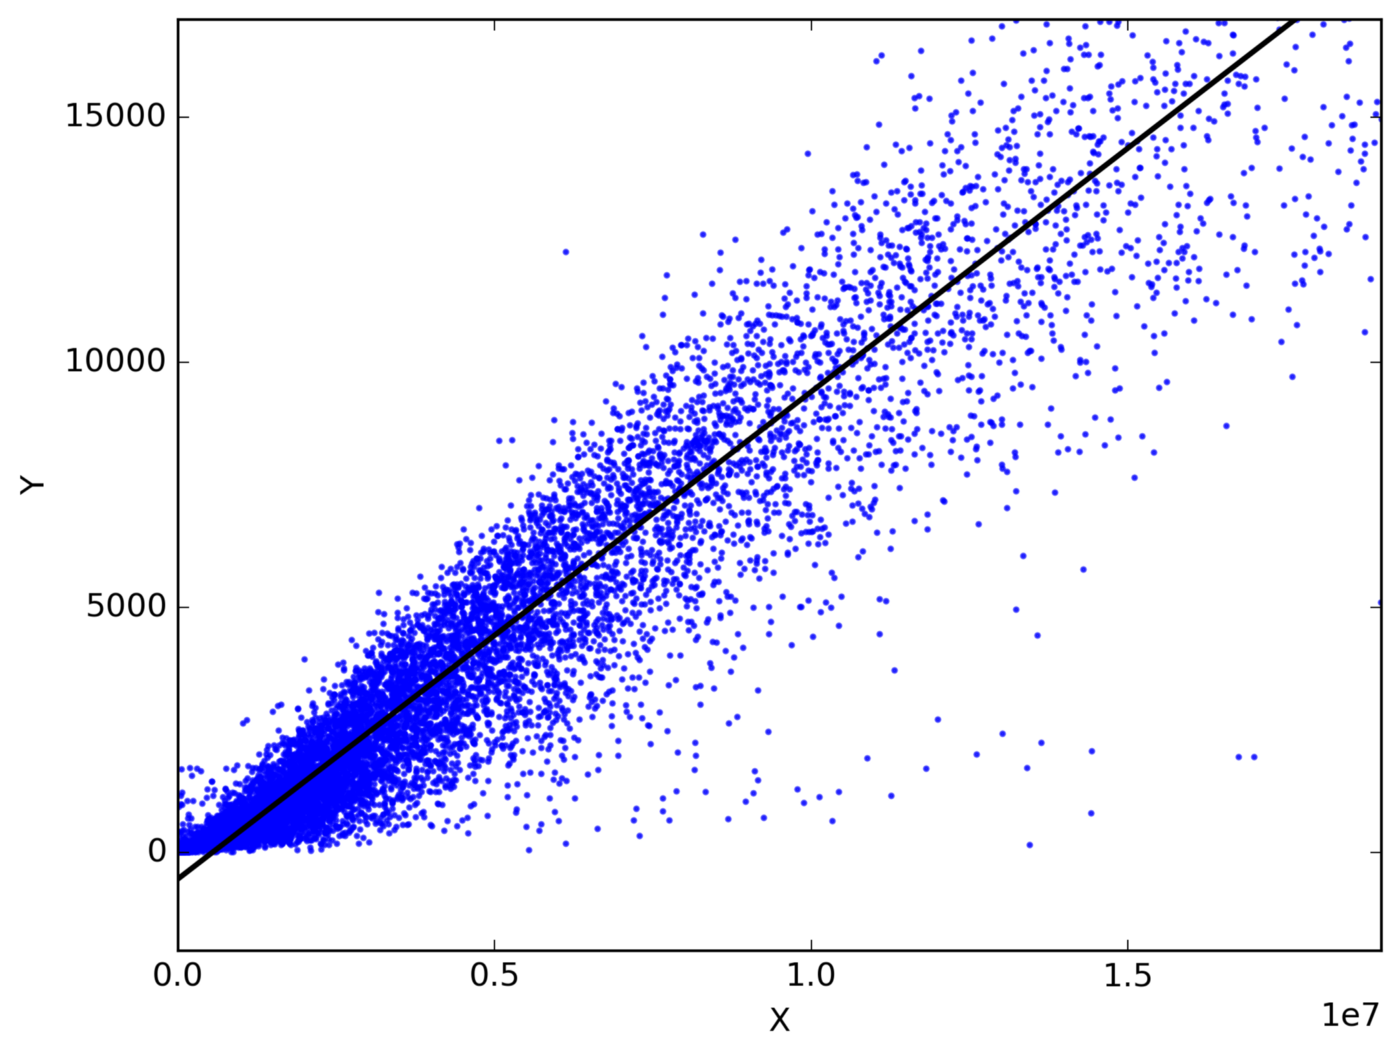
\includegraphics[width=.6\paperwidth]{regression.png}
	\end{center}
\end{frame}

\begin{frame}{Cuadrados Mínimos}
Dado un conjunto de datos $D = {D_1, D_2, \dots, D_k}$, de la forma $D_i = (x_i, y_i)$, donde $x_i \in \mathbb{R}^n$ y $y_i \in \mathbb{R}$, obtener un mapeo lineal $f: X \rightarrow Y$ tal que $f(x_i) = y_i$, $\forall i$.

Como no suele existir, se propone $f(x) = w_1x_1 + w_2x_2 + \dots + w_nx_n + b$ y se busca:

$$
\min_w \sum_{i=1,\dots,n}(y_i - f(x_i))^2
$$

\end{frame}

\begin{frame}{Clustering}
	\begin{center}
	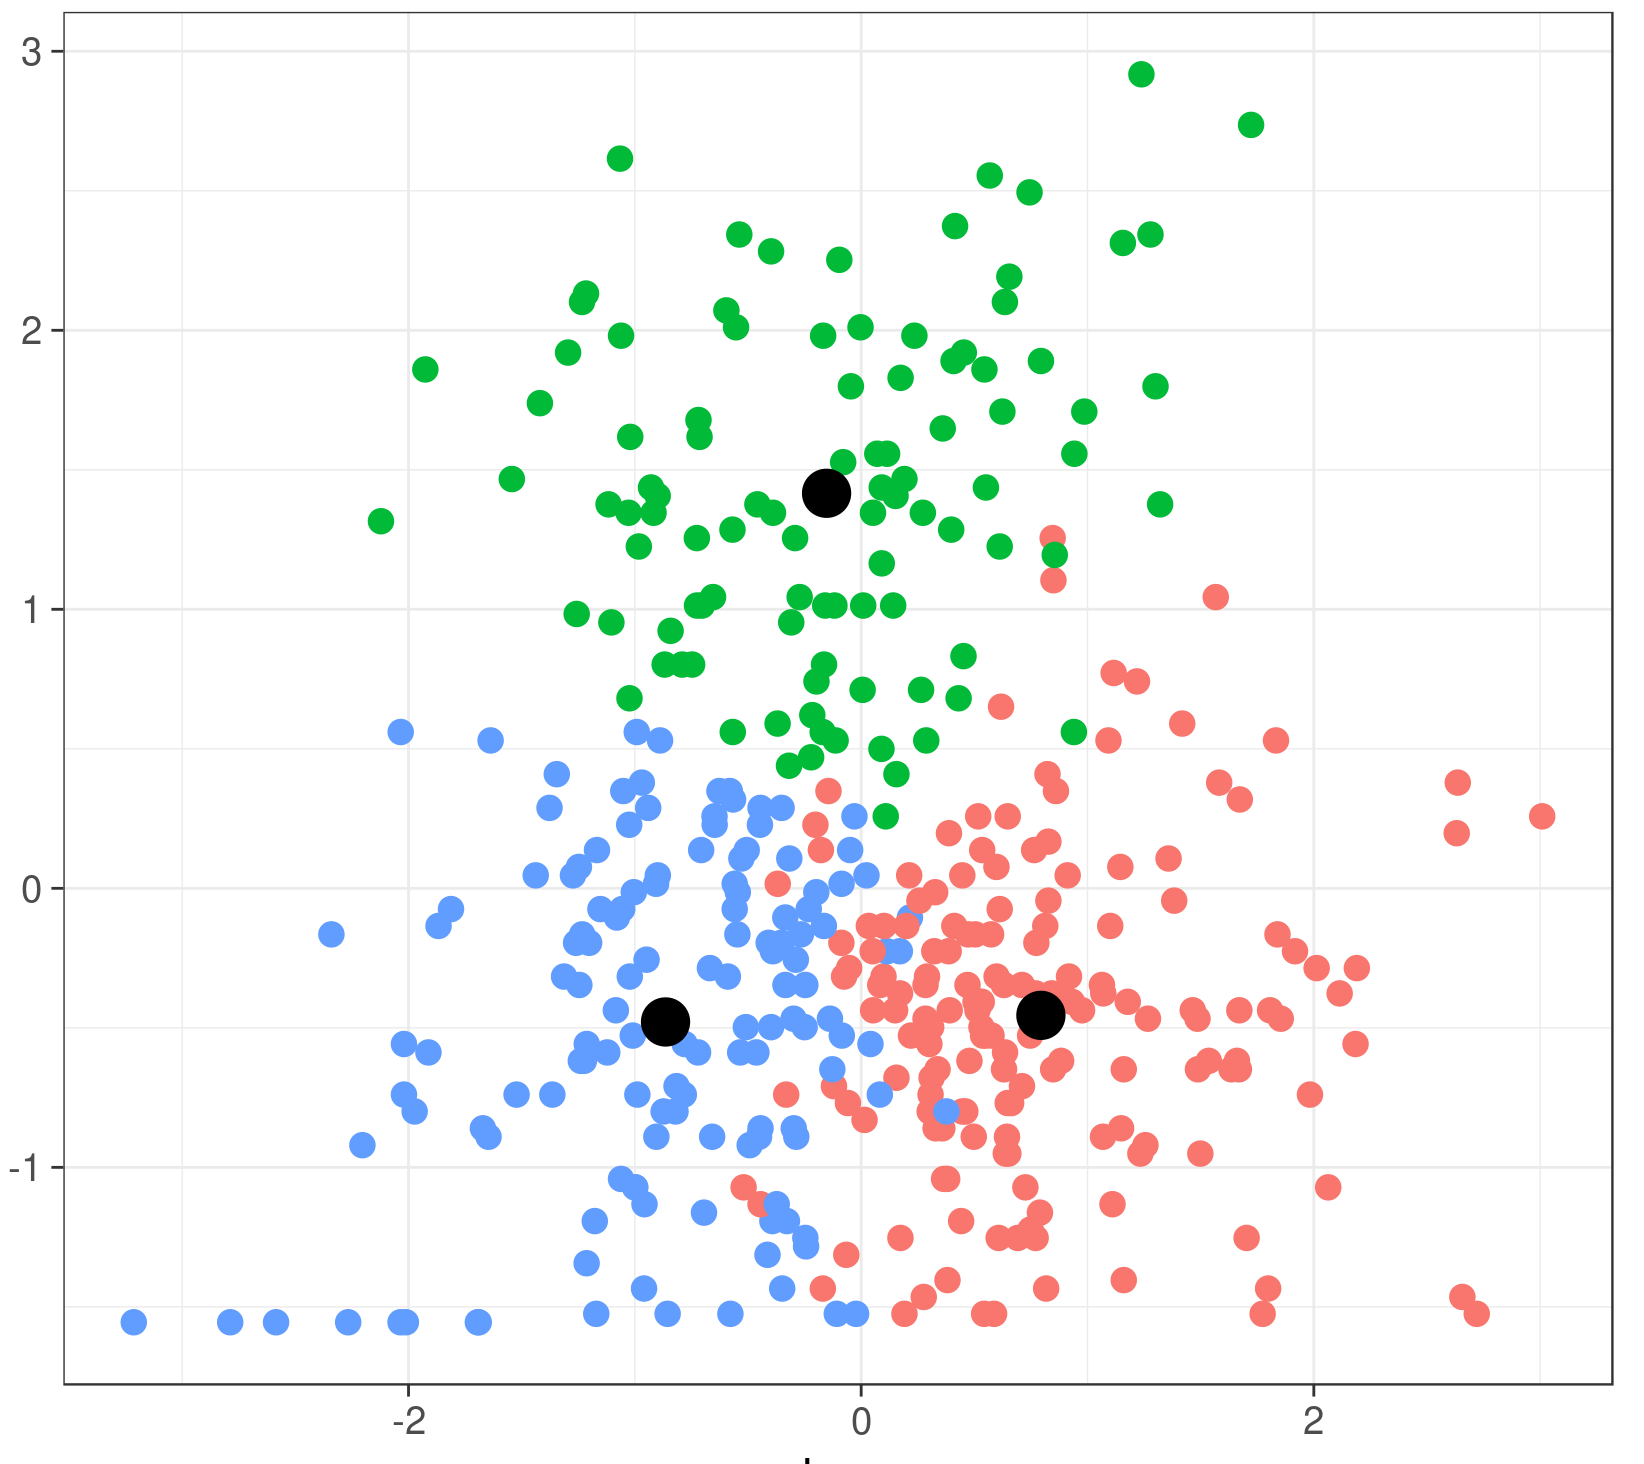
\includegraphics[width=.5\paperwidth]{kmeans.png}
	\end{center}

\end{frame}

\begin{frame}{K-Means}
Dado un conjunto de observaciones $(x_1, x_2, \dots, x_n)$ con $x_i \in \mathbb{R}^n$, particionarlo en $k$ conjuntos $S = {S_1, S_2, \dots, S_k}$

Es un algoritmo iterativo, en cada iteración se propone una partición S y se va corrigiendo, buscando la solución al problema:

$$
argmin_S \sum_{i=1}^{k}\sum_{x \in S_i} \|x-\mu_i\|^2 =
argmin_S \sum_{i=1}^{k}\#S_i Var(S_i)
$$

\end{frame}

\begin{frame}{Sistemas de Recomendación}
	\begin{center}
		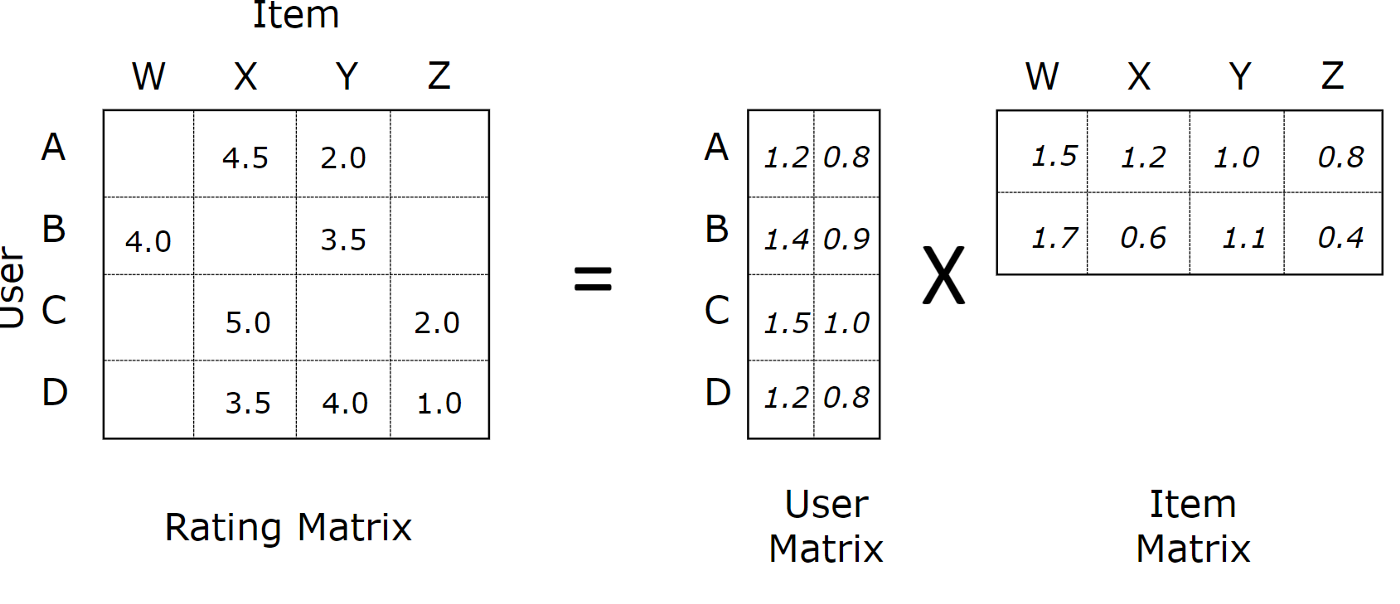
\includegraphics[width=.8\paperwidth]{recommendermatrix.png}
	\end{center}
\end{frame}

\begin{frame}{Factorización de matrices incompletas}

	Dada una matriz $A$ ``con huecos", encontrar la descomposición de la misma en un conjunto de dos matrices más pequeñas, $U$ y $V$, que representen a los usuarios e items, respectivamente y tal que $A = U V^T$.
	
	Si $r_{u,i} = \hat{u}_u^T\hat{v}_i$ y $K$ es el conjunto de observaciones:
	
	$$
	\min_{u\star, v\star} \sum_{(u,i) \in K}c_{u,i}(r_{u,i} - u_u^Tv_i)^2 + \lambda (\|u_u\|^2 + \|v_i\|^2)
	$$
	
\end{frame}

\begin{frame}{Redes Neuronales}
\begin{center}
	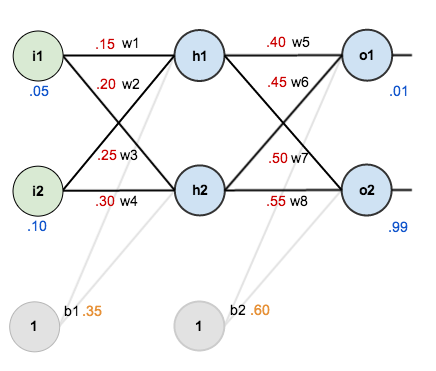
\includegraphics[width=.5\paperwidth]{neuralnet.png}
\end{center}
\end{frame}

\begin{frame}{Back Propagation}

\begin{itemize}
\item La red neuronal no deja de ser una función $F: X \rightarrow Y$ que lleva el input hacia el output.
\item Se puede pensar como una cadena de cuadrados mínimos, donde la aproximación no es necesariamente lineal.
\item La agrupación de capas hace que el modelo \textit{aproxime la realidad} de forma más compleja.
\end{itemize}

$$
F(x_i) = f_1(f_2(\dots(f_n(x_u))))
$$
Luego, buscamos:
$$
\min_w \sum_{i=1,\dots,n}E(y_i - F(x_i))^2
$$

\end{frame}

\begin{frame}{Cómo resolver estos problemas?}
\begin{itemize}
\item Optimización Continua.
\item Función objetivo derivable, conjunto ``amigable"...
\item A seguir el gradiente! (solvers)
\end{itemize}

\begin{center}
	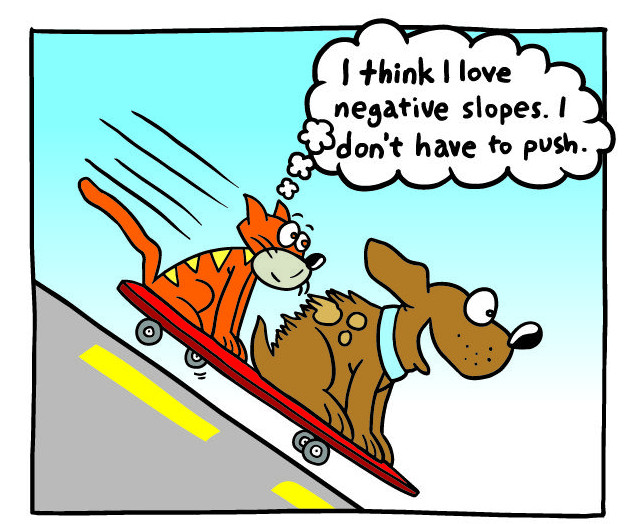
\includegraphics[width=.35\paperwidth]{slope.jpg}
\end{center}
\end{frame}

\begin{frame}{Todo muy lindo, pero...}
	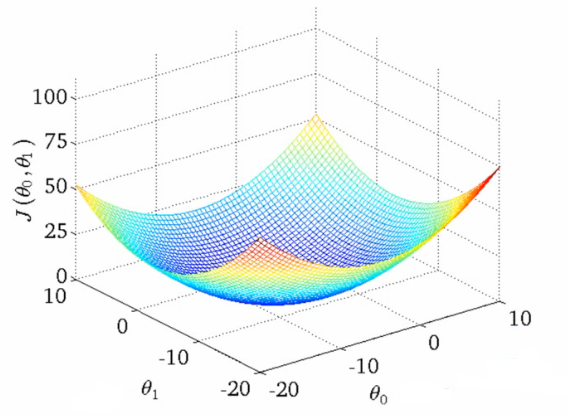
\includegraphics[height=.6\paperheight]{convexopt.png}
	\uncover<2>{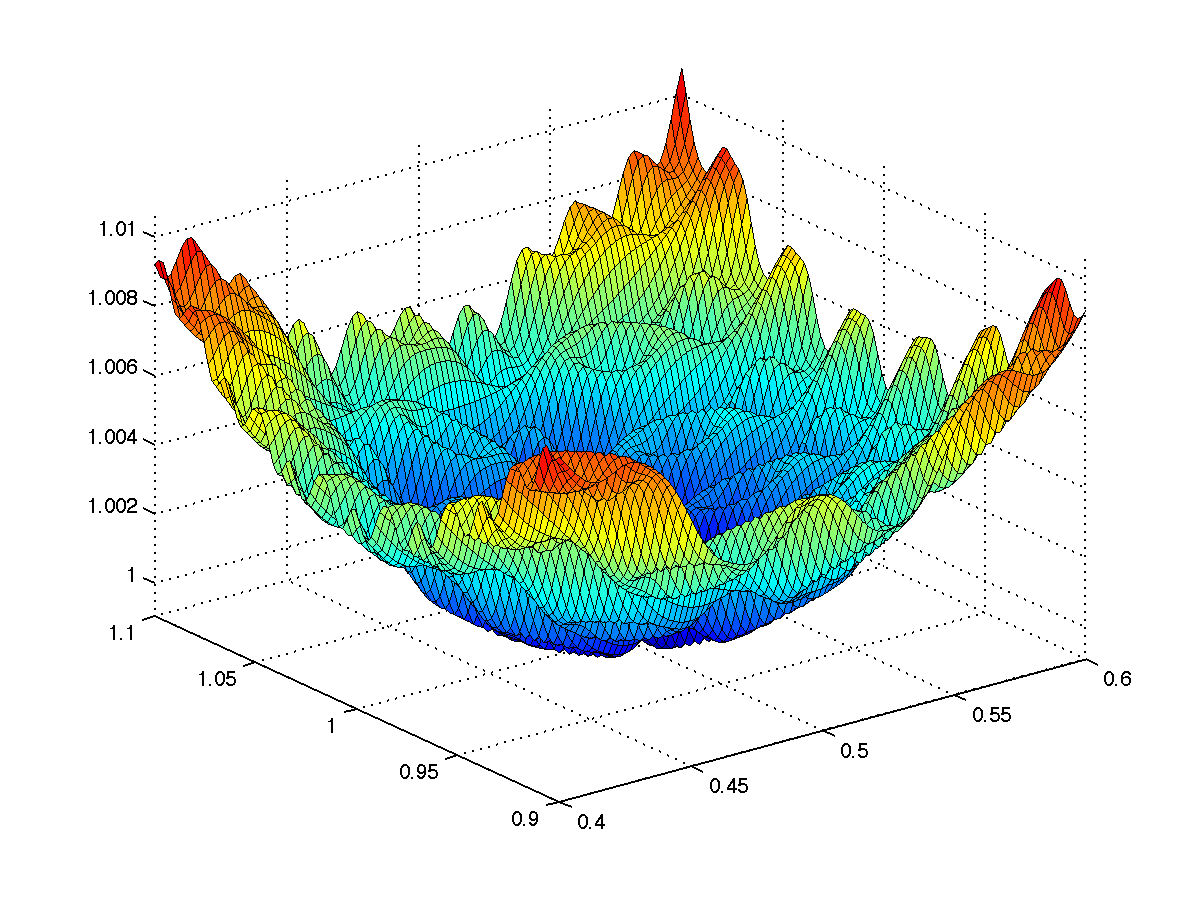
\includegraphics[height=.6\paperheight]{globalopt.png}}
\end{frame}

\begin{frame}{Todo muy lindo, pero...}
\begin{center}
	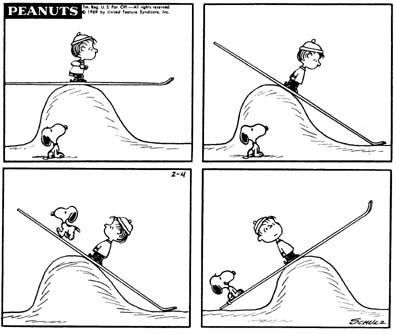
\includegraphics[width=.5\paperwidth]{peanutsslope.jpg}
\end{center}
\end{frame}

\begin{frame}{Más complicaciones...}
\begin{center}
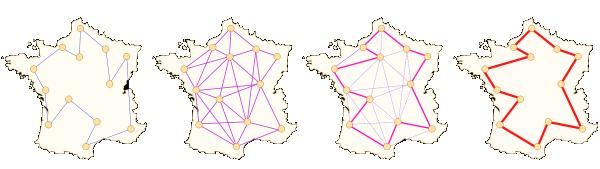
\includegraphics[width=.8\paperwidth]{travelling.jpg}
\end{center}
\end{frame}

\begin{frame}{... llevan a más aplicaciones}
\begin{itemize}
\item Ubicación de antenas de telefonía.
\item Producción de energía mediante diferentes fuentes. (Optimización Estocástica)
\item Diseño de alas de avión. (Optimización de Formas)
\item Funcionamiento correcto de líneas de ensamble. (Investigación Operativa)
\item Planificación de turnos. (Optimización Entera)
\item Armado de fixtures.
\end{itemize}
\end{frame}

\begin{frame}{Para optimizar necesitamos...}
Un Solver:
\begin{itemize}
\item GUROBI
\item CPLEX
\item IPOP
\item Adam - Adadelta, etc.
\end{itemize}

Un Framework que permita aplicarlo:
\begin{itemize}
\item CVXPY (\href{http://www.cvxpy.org/}{http://www.cvxpy.org/})
\item PULP (\href{https://pythonhosted.org/PuLP/}{https://pythonhosted.org/PuLP/})
\item PyOmo (\href{http://www.pyomo.org/}{http://www.pyomo.org/})
\item \textbf{scipy.optimize} (\href{https://docs.scipy.org/doc/scipy/reference/optimize.html}{https://docs.scipy.org/doc/scipy/reference/optimize.html})
\end{itemize}
\end{frame}

\section{Un poco de finanzas}

\begin{frame}{Algunos conceptos básicos}
\begin{itemize}
\item[Acción:] Un activo financiero que representa la tenencia de una fracción del capital de una empresa. Es probablemente el activo más popular a nivel mundial.

\item[Mercado:] Intermediario que permite la interacción de compradores y vendedores de algún tipo de activo financiero.

\item[ByMA:] El mercado minorista de compra/venta de acciones de Argentina.

\item[Merval:] Índice financiero que representa el rendimiento de las acciones más operadas en Argentina.

\item[Portfolio:] Conjunto de inversiones de un individuo.
\end{itemize}
\end{frame}

\begin{frame}{Acciones}
\begin{center}
	
\includegraphics[width=.6\paperwidth]{stock.jpg}
\end{center}
\end{frame}

\begin{frame}{Acciones}
	\begin{center}
		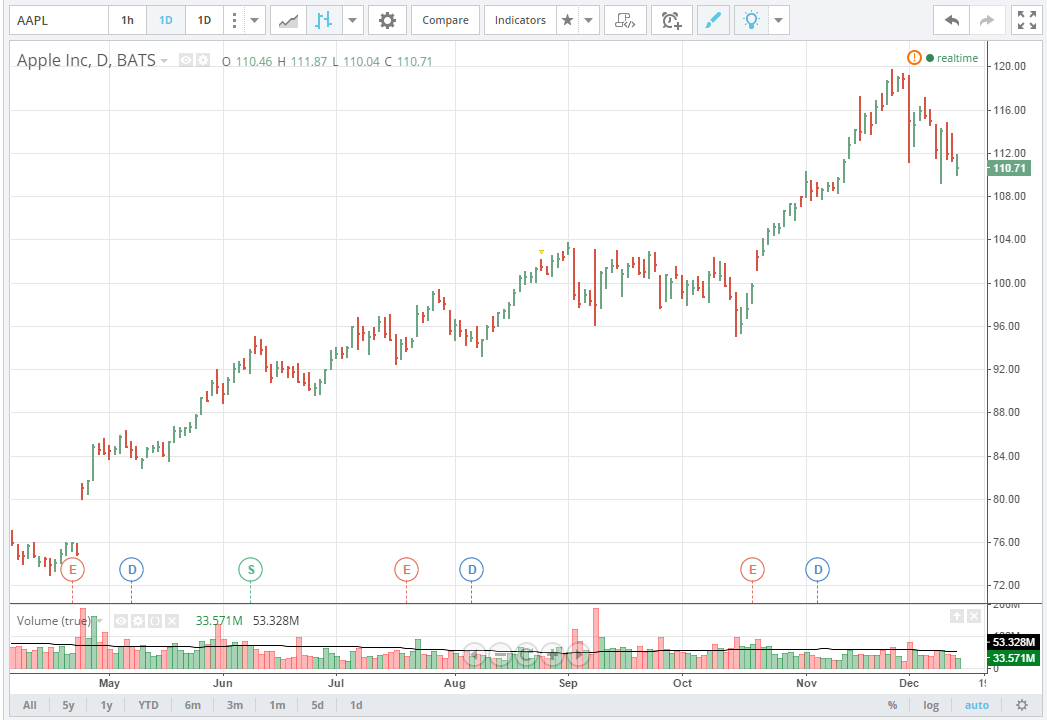
\includegraphics[width=.65\paperwidth]{tradingview.png}
	\end{center}
\end{frame}

\begin{frame}{Qué afecta al valor de una acción?}
\begin{itemize}
\item Bienes y Ganancias.
\item Generación de valor a futuro.
\item Precio de materias primas.
\item Administración de la empresa.
\item Contexto nacional e internacional.
\item ?
\end{itemize}
\end{frame}

\begin{frame}{Qué afecta al valor de una acción?}
\begin{center}
	
\includegraphics[width=.5\paperwidth]{microsoftbusiness.png}
	
	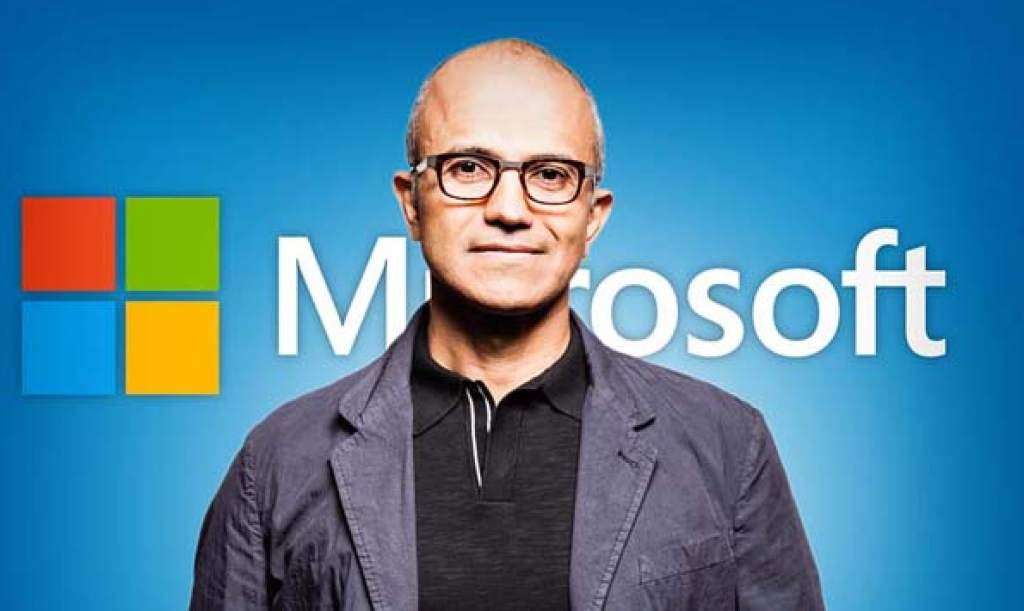
\includegraphics[width=.5\paperwidth]{satyanadella.jpeg}
\end{center}
\end{frame}


\begin{frame}{Qué afecta al valor de una acción?}
\begin{center}
	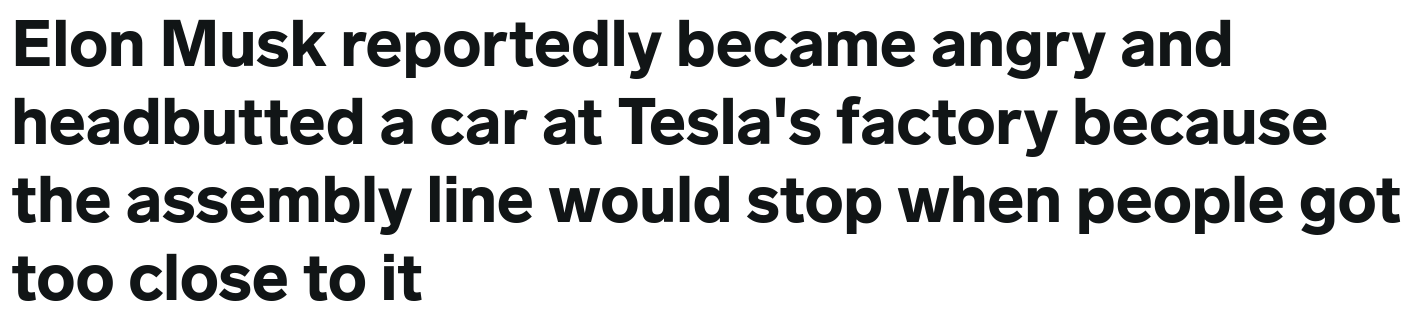
\includegraphics[width=.65\paperwidth]{elonbusiness.png}

	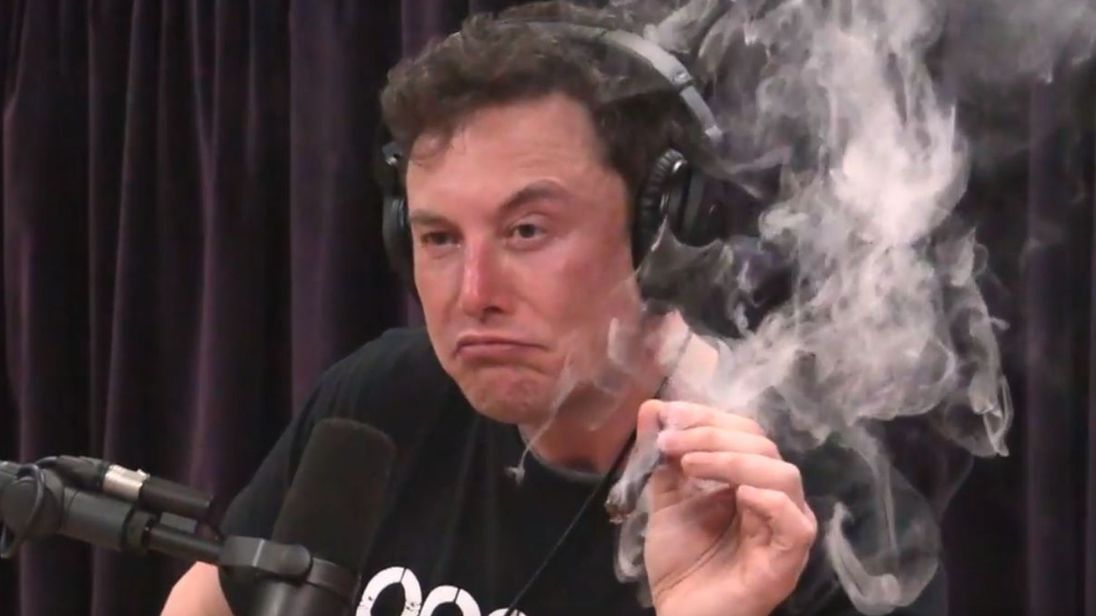
\includegraphics[width=.5\paperwidth]{elonweed.jpg}
\end{center}
\end{frame}

\subsection{Modern Portfolio Theory}

\begin{frame}{Qué es MPT?}
\begin{itemize}
\item Creada por Harry Markowitz en su artículo ``Portfolio Selection" (1952), trabajo por el cual ganó un Premio Nobel en Economía.

\item Asumimos que una persona que invierte en el mercado de capitales quiere maximizar su ganancia esperada.

\item Los mercados a veces son impredecibles y la persona que invierte, además, tiene cierta aversión al riesgo.

\item ``Diversification is the only free lunch in finance".

\item El objetivo para una buena inversión: Maximizar la ganancia esperada y minimizar la variación en el tiempo de la inversión.
\end{itemize}
\end{frame}

\begin{frame}{No poner todos los huevos en una canasta}
\begin{center}
	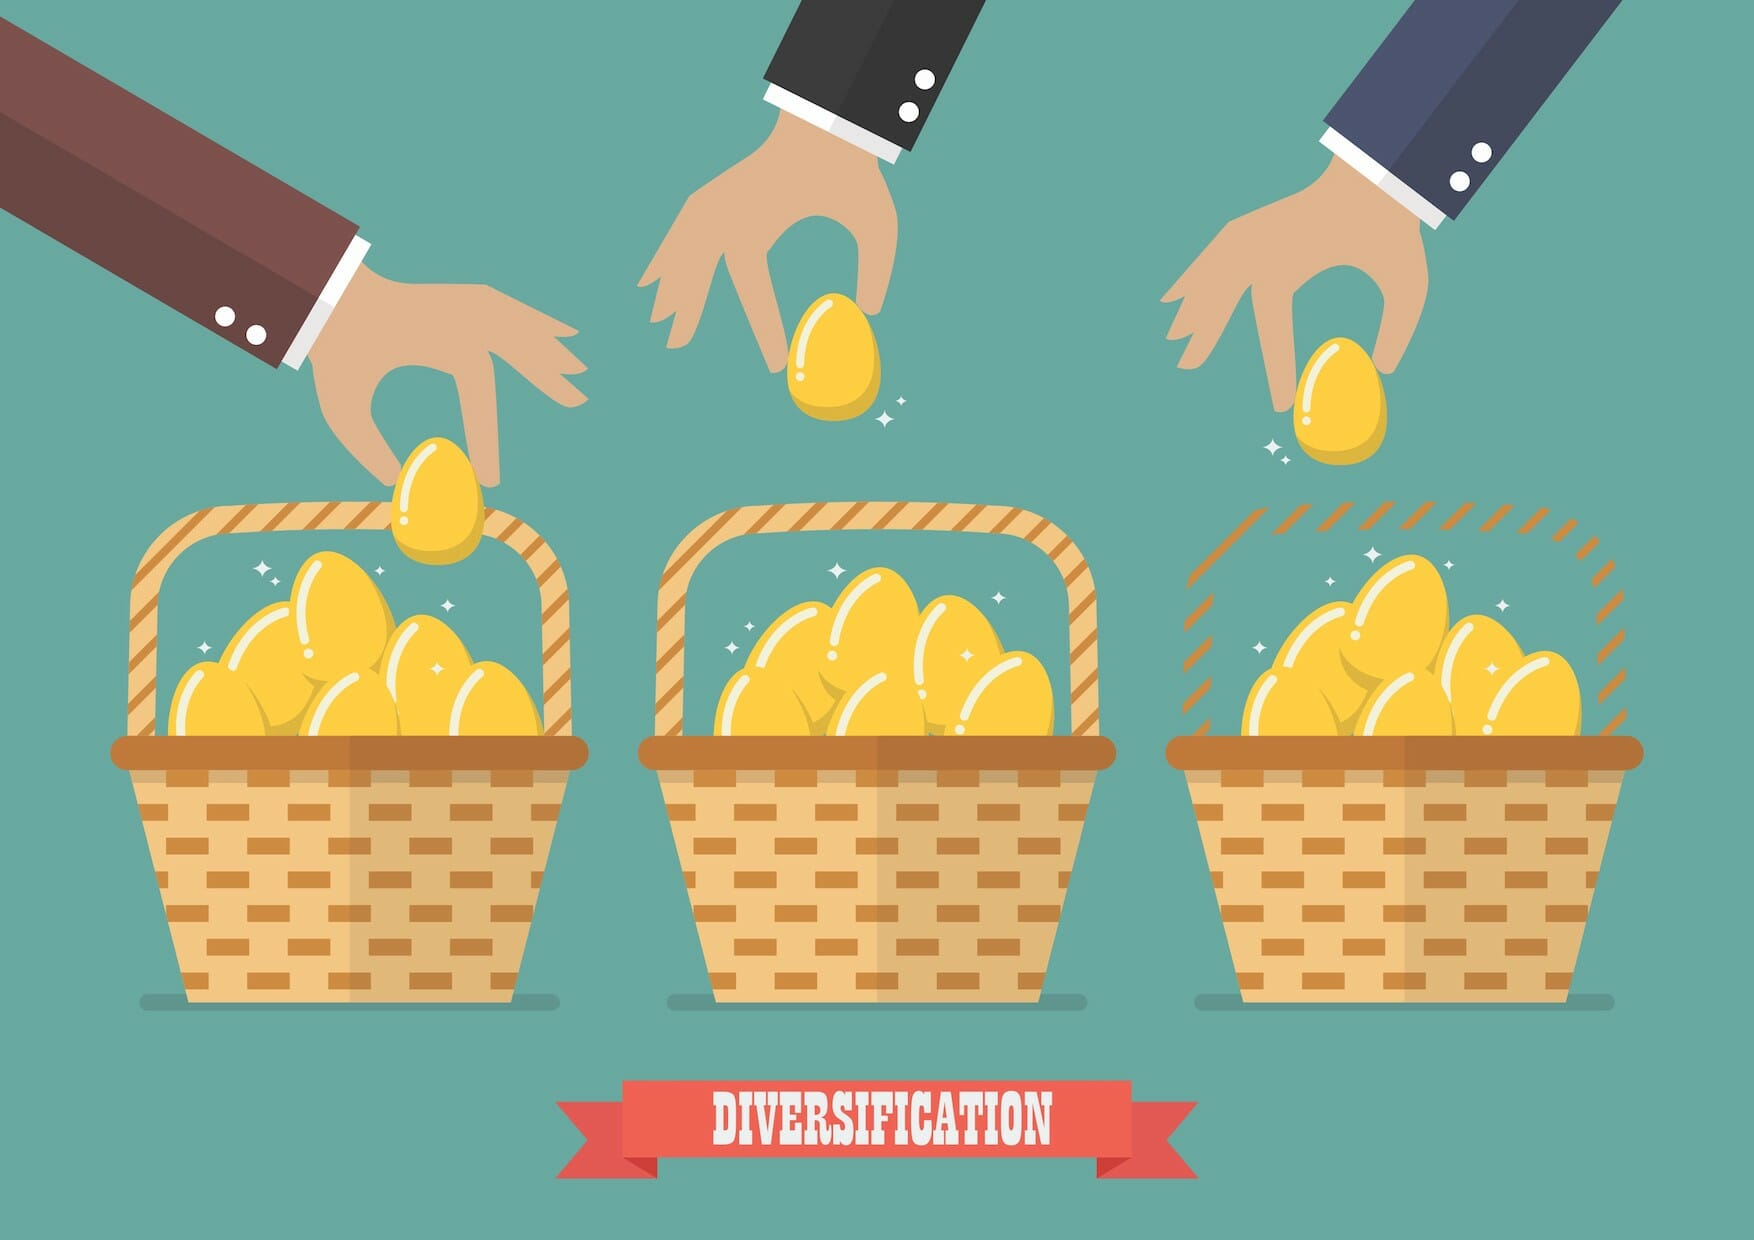
\includegraphics[width=.65\paperwidth]{diversification.jpg}
\end{center}
\end{frame}

\section{Notebook}

\begin{frame}{Datos}
\begin{center}
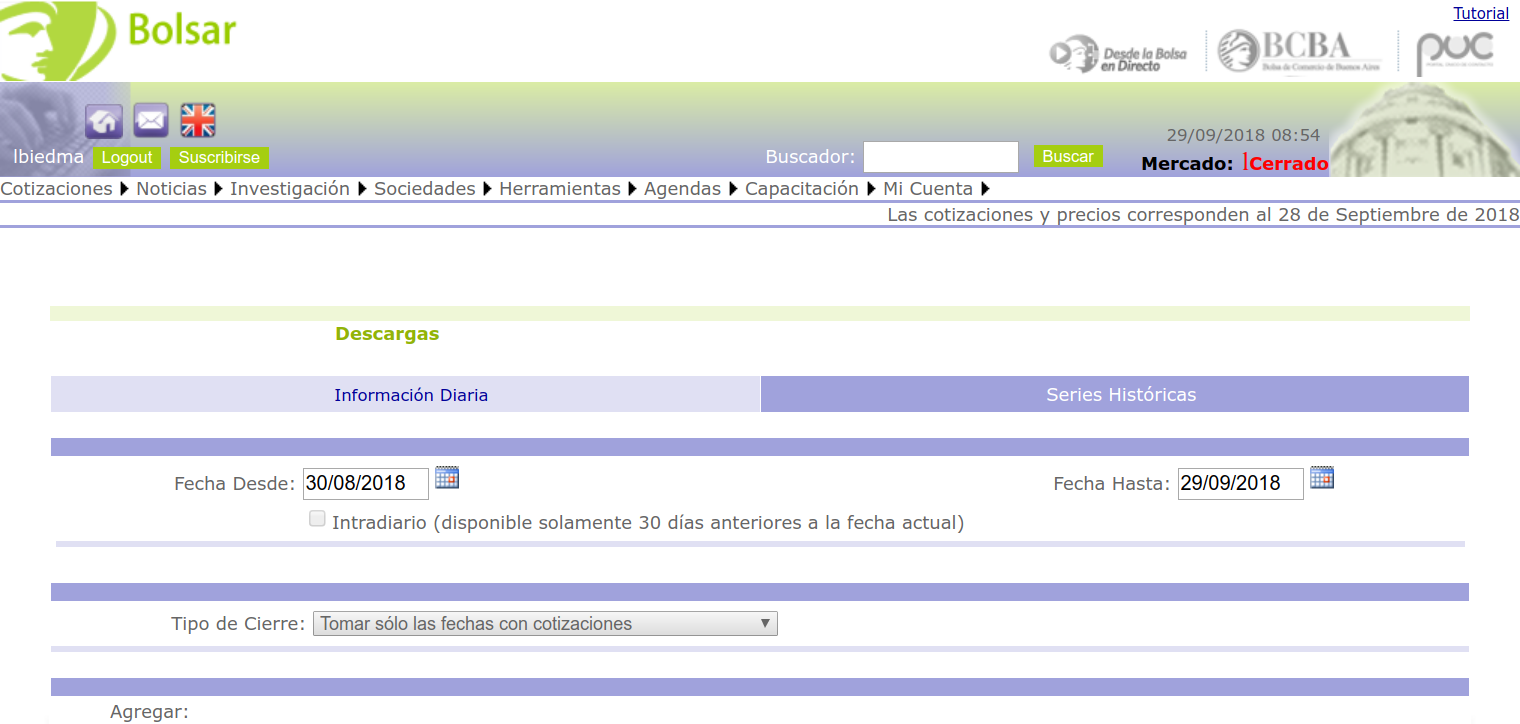
\includegraphics[width = .7\paperwidth]{bolsar.png}
\end{center}
\end{frame}

\begin{frame}{Modelemos nuestro problema}
\begin{itemize}
\item $W = (w_1, w_2, \dots, w_n)$ es el vector de los pesos que le asignemos a cada acción en la que se puede invertir.
\item $E(x_i^d)$ es la ganancia esperada de la acción $i$ el día $d$, entonces $E(X^d)$ es el vector de ganancias esperadas el día $d$.
\item $Cov(X^d)$ es la matriz de covarianza de las variaciones de los precios de las acciones para cada día.
\item $\lambda$ es la aversión al riesgo, es un número real positivo.
\end{itemize}

\uncover<2>{La función a maximizar cada día, para $n$ acciones, es:

$$
f^d(W) = \sum_{i=1}^{n} E(X^d)^T W - \lambda W^T Cov(X^d) W
$$}


\end{frame}

\begin{frame}{Restricciones}
	\begin{itemize}
	\item No podemos invertir más dinero del que tenemos y no podemos vender acciones que no tenemos: $0 \le w_i \le 1$.
	\item Queremos invertir siempre todo el capital que tenemos: $\sum_{i=1}^{n} w_i = 1$.
	\end{itemize}

\begin{center}
	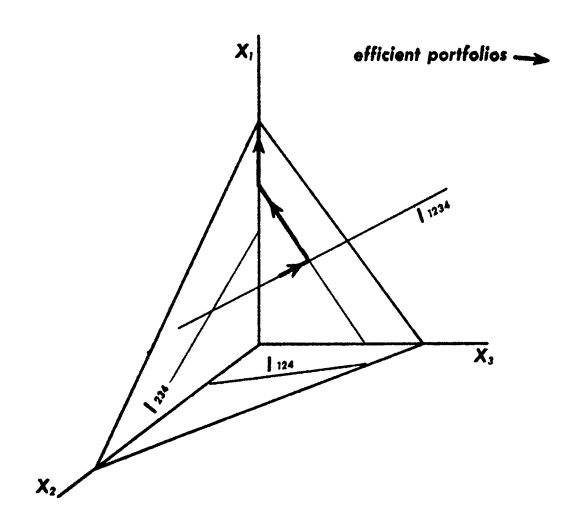
\includegraphics[width=.3\paperwidth]{constraints.png}
\end{center}

\end{frame}


\section{Conclusiones}
\begin{frame}
\textbf{Control de daños:}

\begin{itemize}
\item Le ganamos al mercado!
\item Es posible armar una estrategia de esta manera? Variables enteras...
\item El mercado es MUCHO más grande.
\item Comisiones...
\end{itemize}

\textbf{Espacio para mejorar:}

\begin{itemize}
\item Ganancia esperada.
\item Reinforcement learning.
\item Sentiment analysis
\item Etece, etece, etece...
\end{itemize}
\end{frame}

\begin{frame}
\centering
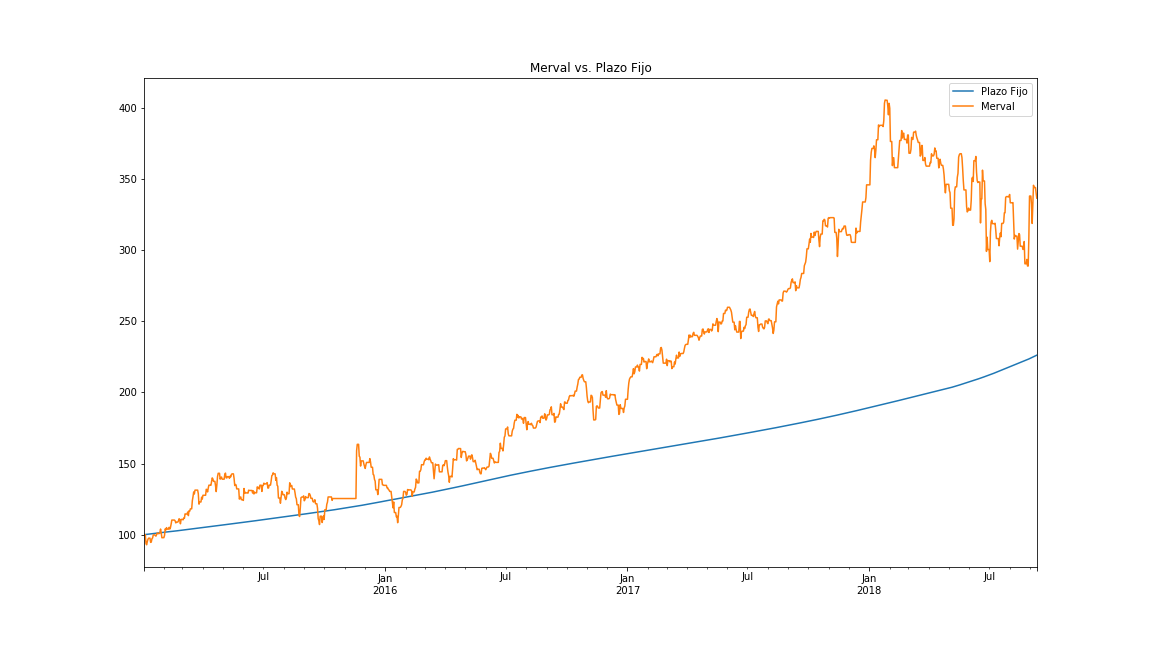
\includegraphics[height=.9\paperheight]{plazofijovsmerval.png}
\end{frame}

\begin{frame}
	\centering
	\huge Muchas gracias!
\end{frame}

\end{document}